% =============================================================================
% Starter draft -- UET vs RoCE/DCQCN in htsim.
% Numbers come from: fidelityRuns/results (flat + rail, 5 seeds, = the H100 deck).
% Fairness/Jain and degraded-link parts are kept below inside \iffalse ... \fi
% (removed from the PDF, kept for easy revert).  Search for "TODO" before submitting.
% Build:  pdflatex main && bibtex main && pdflatex main && pdflatex main
% =============================================================================
\documentclass[conference]{IEEEtran}
\IEEEoverridecommandlockouts
\usepackage{cite}
\usepackage{amsmath}
\usepackage{graphicx}
\usepackage{booktabs}
\usepackage{multirow}
\usepackage{array}
\usepackage{url}
\usepackage{xcolor}
\usepackage{tikz}
\definecolor{fabric}{HTML}{2F6DA8}
\definecolor{nvl}{HTML}{B4671F}
\graphicspath{{figs/}}
% let full-width floats share a page and fill it, so they don't drift past the references
\renewcommand{\topfraction}{0.9}
% \renewcommand{\dbltopfraction}{0.9}
% at most ~one wide figure per page top, so no page is (almost) only figures
\renewcommand{\dbltopfraction}{0.6}
\renewcommand{\textfraction}{0.07}
\renewcommand{\floatpagefraction}{0.8}
\renewcommand{\dblfloatpagefraction}{0.8}
% \setcounter{dbltopnumber}{2}
\setcounter{dbltopnumber}{1}

\newcommand{\roce}{RoCE/DCQCN}
\newcommand{\uet}{UET}
\newcommand{\todo}[1]{\textcolor{red}{[TODO: #1]}}

\begin{document}

\title{Spray or Pause? A Controlled Simulation Study of\\
Ultra Ethernet Transport and RoCE/DCQCN for AI Cluster Fabrics}

% \author{\IEEEauthorblockN{Anonymous Author(s)}
% \IEEEauthorblockA{\todo{affiliation}}}
\author{\IEEEauthorblockA{Technion -- Israel Institute of Technology}}

\maketitle

% -----------------------------------------------------------------------------
\begin{abstract}
AI clusters are increasingly limited by their network, and two designs compete
for the back-end fabric. RoCE with PFC and DCQCN keeps the fabric
\emph{lossless} and pins each flow to one path. The new Ultra Ethernet
Transport (UET) lets the fabric \emph{drop}: it sprays packets across all
paths, trims on overflow and retransmits quickly. We compare the two in the
htsim packet-level simulator with identical topologies, link speeds and
traffic, on flat fat-trees and on rail-optimized GPU clusters with NVLink.
UET is faster in 90 of 99 flat-fabric configurations, by the widest margin on
permutation traffic. RoCE/DCQCN wins only when a single receiver port is the
bottleneck. The two stacks pay for congestion differently: UET in retransmitted
bandwidth, RoCE/DCQCN in PFC pause time. Rail-optimized placement helps both
and nearly closes the gap on MoE all-to-all. Our results suggest that most of
UET's advantage comes from per-packet spraying rather than from its
loss-recovery design.
\end{abstract}

% previous, more detailed abstract (kept for easy revert)
\iffalse
\begin{abstract}
AI and HPC clusters are increasingly limited by their network, and two design
philosophies now compete for the back-end fabric. RoCE with PFC and DCQCN keeps
the fabric \emph{lossless} and pins each flow to one ECMP path. The new Ultra
Ethernet Transport (UET) lets the fabric \emph{drop}, sprays every packet across
all paths, trims overflowing packets, and retransmits quickly. We compare the two
in the htsim packet-level simulator under identical topologies, link speeds and
traffic matrices. The study covers 400\,Gb/s fat-trees of 128 and 1024 nodes at
three oversubscription ratios, rail-optimized clusters of 1024 and 2048 GPUs
with an NVLink domain, and seven workload patterns, for 1{,}635 simulations in
total. UET finishes faster in 90 of 99 flat-fabric configurations: a median
3.3$\times$ on permutation traffic, about 1.3$\times$ on incast and 2$\times$
on ring all-reduce. RoCE/DCQCN wins only on 1024-node incast, where the receiver
port is the bottleneck. The two stacks pay for congestion differently. UET
spends bandwidth, trimming up to 62\% of transmissions in an oversubscribed
all-to-all. RoCE/DCQCN spends time, with up to
3{,}350 port-seconds of PFC pause, and never drops a packet. On GPU clusters
with an NVLink domain, rail-optimized placement helps both stacks, RoCE/DCQCN
by 8--41\% and UET by 3--10\%, and brings RoCE/DCQCN to within
1.02--1.33$\times$ of UET on MoE all-to-all.
% removed: "We also report and fix nine defects in htsim's DCQCN implementation."
% removed: "...all-to-all, and its fairness collapses there." and
% "Finally, when a single fabric link degrades to 10\% of its speed, RoCE/DCQCN
% slows by up to 8.2$\times$ while UET slows by at most 1.35$\times$."
\end{abstract}
\fi

\begin{IEEEkeywords}
Ultra Ethernet, RoCE, DCQCN, PFC, packet spraying, datacenter networks,
AI training, collective communication, htsim
\end{IEEEkeywords}

% -----------------------------------------------------------------------------
\section{Introduction}

Distributed training and inference are dominated by collective communication:
all-reduce for gradient synchronization, all-to-all for Mixture-of-Experts (MoE)
routing, and many-to-one gathers. These patterns are bursty and synchronized,
and they create exactly the congestion that commodity datacenter transports
handle worst. The back-end fabric therefore matters for end-to-end job time.

Two philosophies compete for that fabric. The incumbent, RDMA over Converged
Ethernet (RoCEv2), relies on Priority Flow Control (PFC)~\cite{pfc} to make the
network lossless. DCQCN~\cite{dcqcn} slows senders before buffers fill. Because
RoCE expects near-in-order delivery, each flow is pinned to a single ECMP path.
The Ultra Ethernet Consortium's transport (UET)~\cite{uec-spec,uec-design}
takes the opposite approach. It tolerates loss instead of preventing it. Every
packet is sprayed across all paths, switches \emph{trim} rather than drop
overflowing packets~\cite{ndp} so that the receiver can request a fast
retransmission, and a sender-based congestion controller (NSCC) reacts to delay
and ECN.

Which approach is better, on which traffic, and at what cost? Vendor results
are hard to compare because they change the transport, the topology and the
hardware all at once. We instead implement both stacks in one packet-level
simulator, htsim~\cite{ndp}, and change only the transport. Our contributions:

\begin{itemize}
  \item \textbf{A controlled comparison} of UET and RoCE/DCQCN on 400\,Gb/s
        fat-trees (128 and 1024 nodes, 1:1/4:1/8:1 oversubscription) across
        seven traffic patterns. Every configuration is repeated with five ECMP
        seeds and every difference is tested for significance (\S\ref{sec:flat}).
  \item \textbf{An accounting of what each stack pays}: retransmitted bandwidth
        for UET, PFC pause time and lower link utilization for
        RoCE/DCQCN (\S\ref{sec:cost}).
  \item \textbf{Rail-optimized GPU clusters with NVLink}, modelled with a
        second, intra-server topology (Fig.~\ref{fig:railtopo}), showing that
        rails help \emph{both} transports and narrow the gap on MoE all-to-all
        (\S\ref{sec:rail}).
\iffalse
  \item \textbf{Robustness to a degraded link}: a single slow fabric link costs
        RoCE/DCQCN up to 8.2$\times$ and UET at most 1.35$\times$
        (\S\ref{sec:degraded}).
\fi
\iffalse
  \item \textbf{A corrected DCQCN model}: we identify and fix nine defects in
        htsim's DCQCN, two of which made its dynamics meaningless
        (\S\ref{sec:dcqcn}).
\fi
\end{itemize}

% -----------------------------------------------------------------------------
\section{Background}

\textbf{RoCE, PFC and DCQCN.}
RoCEv2 carries RDMA over UDP/IP. PFC makes a priority class lossless: when an
ingress buffer crosses a threshold, the switch pauses its upstream neighbour.
This avoids loss but can spread congestion to flows that do not use the hot
link (head-of-line blocking, congestion trees)~\cite{rdma-scale}. DCQCN adds
end-to-end rate control. Switches ECN-mark packets above a queue threshold, the
receiver returns congestion notification packets (CNPs), and the sender cuts its
rate multiplicatively, then recovers through timer- and byte-counter-driven
increase stages~\cite{dcqcn}. Each flow follows one ECMP path, so long flows that
hash onto the same link collide for their whole lifetime~\cite{hedera}.

\textbf{Ultra Ethernet Transport.}
UET~\cite{uec-spec,uec-design} targets the same RDMA semantics on a best-effort
Ethernet fabric. Its key mechanisms are:
(i) \emph{per-packet spraying} across many paths, selected by an entropy value
in the header~\cite{spray,reps};
(ii) \emph{packet trimming}: an overflowing switch forwards only the header,
which triggers a NACK and a fast retransmit instead of a timeout~\cite{ndp};
(iii) an out-of-order-tolerant receiver; and
(iv) NSCC, a sender-based window controller driven by delay and
ECN~\cite{reps}. UET is a recent standard, and there are still few independent
evaluations of it against the RoCE baseline it aims to replace.

% -----------------------------------------------------------------------------
\section{Methodology}
\label{sec:method}

\subsection{Simulator and stacks}
We use htsim~\cite{ndp}, which includes models of both the UEC transport and
RoCE. Table~\ref{tab:stacks} lists the two configurations. Everything
except the transport is shared: topology files, link speeds, link latencies and
traffic matrices. MTU is each stack's native default (4000\,B for RoCE, 4150\,B
for UET), a difference of a few percent in per-packet overhead. We run UET with
sender-based congestion control only (\texttt{-sender\_cc\_only}), which disables
its optional receiver-credit mode, so neither stack is given knowledge of the
oversubscription.

\begin{table}[t]
\centering
\caption{The two transport stacks. All other parameters are identical.}
\label{tab:stacks}
\footnotesize
\setlength{\tabcolsep}{4pt}
\begin{tabular}{@{}lll@{}}
\toprule
 & \textbf{RoCE/DCQCN} & \textbf{UET} \\
\midrule
Fabric          & lossless (PFC)            & lossy + trimming \\
Load balancing  & per-flow ECMP (128 paths) & per-packet spraying \\
Congestion ctrl & DCQCN, ECN $K{=}8$ pkts   & NSCC (sender-based) \\
Switch buffer   & 1000 pkts/port            & 1$\times$BDP ($\approx$627\,KB) \\
PFC thresholds  & 12 / 15 pkts (ingress)    & --- \\
ECN marking     & single threshold $K$      & 20\% / 80\% of BDP \\
Loss recovery   & go-back-N (never needed)  & NACK on trim, selective \\
MTU             & 4000\,B                   & 4150\,B \\
\bottomrule
\end{tabular}
\end{table}

\iffalse
\subsection{Correcting htsim's DCQCN}
\label{sec:dcqcn}
Before running the RoCE baseline we audited htsim's DCQCN implementation and
found nine defects, all fixed in the version we use:
(1) the rate-reduction factor $\alpha$ was a \emph{static} variable shared by
all flows, so one flow's congestion cut every flow's rate;
(2) there was no minimum rate, so repeated multiplicative cuts truncated the
integer rate to zero and caused a division by zero in pacing, stalling flows
indefinitely under incast;
(3) the byte counter added packets but compared against a byte threshold, so
byte-counter increase and hyper-increase never fired;
(4) the $\alpha$-decay timer was never re-armed, so $\alpha$ decayed on every
event instead of every 55\,$\mu$s and rate cuts effectively vanished;
(5) the completion check compared packets with bytes, so finished senders kept
scheduling events;
(6)--(9) a packet leak after completion, per-link increase constants declared
static, 16-bit timer/byte counters that wrapped after $\approx$3.6\,s, and a
logger type mismatch.
Defects (1), (2) and (4) interact. Making $\alpha$ per-flow and decaying it
correctly makes the cuts real, which makes the zero-rate collapse more likely,
so the rate floor has to be added in the same change. We consider the corrected
model a prerequisite for any htsim study that uses DCQCN as a baseline.
\fi

\subsection{Topologies}
\textbf{Flat fat-trees.}
Three-tier fat-trees of 128 nodes (8 pods of 16) and 1024 nodes (16 pods of
64) with 400\,Gb/s links on every tier and 1\,$\mu$s per-hop latency. We build
oversubscription by removing uplinks, not by slowing them. At 128 nodes the
number of distinct inter-pod paths therefore falls from 16 (1:1) to 4 (4:1) to 2
(8:1). This matters for the interpretation in \S\ref{sec:flat}.

\textbf{Rail-optimized clusters with NVLink.}
1024 and 2048 GPUs as DGX H100-like servers of 8 GPUs, each GPU with its own
400\,Gb/s NIC on its own \emph{rail}, in a two-tier non-blocking leaf-spine with
64-port leaves (32 down, 32 up). A leaf holds one GPU from each of 32 servers. A
\emph{flat control} has the same switches and links but attaches hosts
consecutively, so any difference comes from the host-to-leaf assignment alone. We
model NVLink4 as a second topology: one 3600\,Gb/s crossbar per server with
100\,ns links. Each flow is routed at connection time over NVLink if both
endpoints share a server, and over the rail fabric otherwise. The simulator
checks that each plane's link capacity matches its host injection rate, because
a mismatch silently throttles traffic to the slower of the two.
Fig.~\ref{fig:railtopo} sketches the resulting two-plane cluster.

\begin{figure}[t]
\centering
\resizebox{\columnwidth}{!}{%
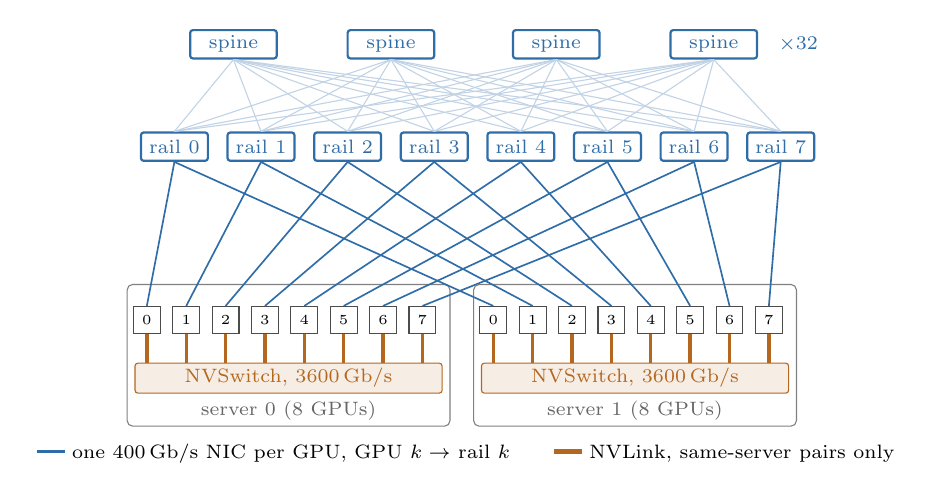
\begin{tikzpicture}[x=1cm,y=1cm,font=\scriptsize,
  sw/.style={draw=fabric,thick,rounded corners=1pt,minimum height=0.36cm,inner sep=1pt,text=fabric},
  gpu/.style={draw=black!70,fill=white,minimum size=0.34cm,inner sep=0pt,font=\tiny}]
  % spines and rail leaves
  \foreach \i/\x in {0/1.2,1/3.2,2/5.3,3/7.3}
    \node[sw,minimum width=1.1cm] (sp\i) at (\x,4.0) {spine};
  \node[anchor=west,text=fabric] at (8.0,4.0) {$\times$32};
  \foreach \k in {0,...,7}
    \node[sw,minimum width=0.85cm] (L\k) at ({0.45+\k*1.1},2.7) {rail \k};
  \foreach \k in {0,...,7}
    \foreach \i in {0,...,3}
      \draw[fabric!30] (L\k.north) -- (sp\i.south);
  % two servers of 8 GPUs; GPU k of every server goes to rail k
  \foreach \s in {0,1} {
    \draw[black!50,rounded corners=2pt] ({\s*4.4-0.15},-0.85) rectangle ({\s*4.4+3.95},0.95);
    \node[anchor=south,inner sep=2pt,text=black!60] at ({\s*4.4+1.9},-0.85) {server \s{} (8 GPUs)};
    \foreach \k in {0,...,7} {
      \node[gpu] (g\s\k) at ({\s*4.4+0.1+\k*0.5},0.5) {\k};
      \draw[fabric,semithick] (g\s\k.north) -- (L\k.south);
      \draw[nvl,very thick] (g\s\k.south) -- ++(0,-0.38);
    }
    \draw[nvl,fill=nvl!12,rounded corners=1pt] ({\s*4.4-0.05},-0.43) rectangle ({\s*4.4+3.85},-0.05);
    \node[text=nvl] at ({\s*4.4+1.9},-0.24) {NVSwitch, 3600\,Gb/s};
  }
  \node[align=center] at (4.15,-1.2)
    {\textcolor{fabric}{\rule[2pt]{10pt}{1pt}}~one 400\,Gb/s NIC per GPU, GPU $k\to$ rail $k$\qquad
     \textcolor{nvl}{\rule[1.5pt]{10pt}{2pt}}~NVLink, same-server pairs only};
\end{tikzpicture}}
\caption{The rail-optimized cluster with NVLink (two of 128/256 servers shown;
one leaf drawn per rail, 4 or 8 in the real cluster). Every GPU has two egress
planes. A flow between GPUs of the same server is routed over the server's
NVLink switch; any other flow uses the rail fabric, where GPU $k$ of every
server attaches to a leaf of rail~$k$. The flat control keeps the same switches
but attaches whole servers to consecutive leaves.}
\label{fig:railtopo}
\end{figure}

\subsection{Workloads}
Table~\ref{tab:workloads} summarizes the traffic. Flat-fabric patterns use flow
sizes of 16, 64 and 100\,MB. All-to-all and ring all-reduce were run at 128
nodes only, because the 1024-node versions exceeded our memory budget. Ring
all-reduce and the rail-aware collectives are \emph{trigger-chained}: a flow
starts when its predecessor finishes, so flow completion time (FCT) includes
waiting time and only the makespan is comparable across them.

\begin{table}[t]
\centering
\caption{Workloads. $N$ = number of nodes, $S$ = flow size.}
\label{tab:workloads}
\small
\begin{tabular}{@{}>{\raggedright\arraybackslash}p{0.29\columnwidth}>{\raggedright\arraybackslash}p{0.63\columnwidth}@{}}
\toprule
\textbf{Pattern} & \textbf{Definition (what it mimics)} \\
\midrule
Permutation (random) & $N$ flows, random permutation (shuffle traffic) \\
Permutation (full-bis.) & node $i \to i{+}N/2$; every flow crosses the bisection \\
Incast (random) & $N{-}1$ senders $\to$ node 0 (storage read, gather) \\
Incast (remote) & far half of the fabric $\to$ node 0 (incast + core) \\
Outcast-incast & $N/8$ senders $\to$ node 0, each also fanning out \\
All-to-all & all $N(N{-}1)$ pairs at once, $S$ per pair \\
Ring all-reduce & trigger-chained ring, 32{,}640 transfers at $N{=}128$ \\
\midrule
Rail all-reduce & NVLink reduce-scatter, rail-local recursive halving/doubling, NVLink all-gather \\
Rail MoE all-to-all & NVLink shuffle to the destination rail, then rail-local all-to-all ($\approx$125\,KB per peer) \\
\bottomrule
\end{tabular}
\end{table}

% float placed early: figure* appears on the next page

\begin{figure*}[!t]
\centering
\includegraphics[width=0.92\textwidth]{f07_ib_uet_ratio_flat.png}
\caption{RoCE/DCQCN makespan divided by UET makespan on the flat fat-tree (mean
of 5 seeds). Values above 1 mean UET is faster. ``IB'' in the figure denotes
RoCE/DCQCN. All 99 comparisons are significant (Welch $p{<}0.05$).}
\label{fig:ratio}
\end{figure*}

\subsection{Metrics and statistics}
\emph{Makespan} (time until the last flow completes) is the headline metric. We
also record FCT percentiles, slowdown (FCT divided by its ideal on an idle
network), and per-tier link utilization.
% removed from the list above: "Jain fairness over per-flow throughput," Each stack's native congestion cost is recorded as well: the trim
rate NACKs/(new\,+\,retransmitted) for UET, and PFC pause count, pause time and
peak buffer occupancy for RoCE/DCQCN. A lossless run that ever exceeds its
buffer is flagged as misconfigured rather than reported. Across all 660 RoCE runs
none did.

htsim is deterministic for a fixed seed. The seed sets each switch's ECMP hash
salt and path permutation, so each seed is an equally valid draw of where flows
land. Flat-fabric and rail results are the mean of five seeds (1{,}275 and 240
runs). Stack comparisons use Welch's $t$-test at $p{<}0.05$.
% removed: "The degraded-link study (\S\ref{sec:degraded}) uses one seed and
% reports effect sizes far above the seed-to-seed variation of the same configurations."

% -----------------------------------------------------------------------------
\begin{figure*}[!t]
\centering
% was: stacked at 0.78\textwidth each (made a near figure-only page)
\includegraphics[width=0.495\textwidth]{f02_uet_trim_rate_os_128.png}\hfill
\includegraphics[width=0.495\textwidth]{f03_ib_pfc_pause_os_1024.png}
\caption{The two currencies of congestion. Left: UET trim rate (\% of all
transmissions) at 128 nodes. Right: RoCE/DCQCN cumulative PFC pause time at
1024 nodes. Mean $\pm$ 95\% CI over 5 seeds.}
\label{fig:cost}
\end{figure*}

\section{Results}

\subsection{Speed on the flat fabric}
\label{sec:flat}


Fig.~\ref{fig:ratio} shows the ratio of RoCE/DCQCN to UET makespan for every
flat-fabric configuration. All 99 differences are statistically significant.
UET is faster in 90.

\textbf{Permutation: the load-balancing gap.}
The largest gap is on permutation traffic: a median of 3.3$\times$, with a range
of 1.9--8.5$\times$. UET comes close to the line-rate bound. A 16\,MB permutation at 128 nodes
completes in about 400\,$\mu$s against an ideal of 320\,$\mu$s, while
RoCE/DCQCN needs about 2.6\,ms. Spraying spreads every flow over all
paths. Per-flow ECMP instead lets several flows hash onto one link, and those
flows then share it for their whole lifetime.

\textbf{Oversubscription shrinks the gap.}
At 128 nodes and 16\,MB the permutation ratio falls from 6.65$\times$ (1:1) to
3.36$\times$ (4:1) to 2.43$\times$ (8:1). The same trend holds at every size and
at 1024 nodes. Because we oversubscribe by removing uplinks, path diversity
collapses at the same time: from 16 inter-pod paths to 2. With fewer paths to
spray across, spraying gains less over hashing. The gap that remains at 8:1 is
an upper bound on what the transport alone (trimming and NSCC versus PFC and
DCQCN) contributes on this pattern. This suggests that most of UET's
permutation advantage at full bisection comes from load balancing, not from the
loss-recovery design. A direct ablation is future work (\S\ref{sec:discussion}).

\textbf{Incast and collectives.}
On incast and outcast-incast UET is about 1.3$\times$ faster (median), and the
ratio barely changes with oversubscription: the receiver's downlink, not the
core, is the bottleneck. All-to-all goes from 1.52$\times$ at 1:1 to
1.03$\times$ at 8:1, and ring all-reduce from 3.40$\times$ to 1.79$\times$.

\textbf{Where RoCE/DCQCN wins.}
All nine RoCE/DCQCN wins are incast at 1024 nodes: 3--7\% on random incast and
about 0.5\% on remote incast. There, 1023 senders converge on one port, so
spraying has nothing to spread. UET then pays for its loss-based design: at
1024 nodes, 75--84\% of its random-incast transmissions are trimmed, and most
packets are sent more than once. PFC instead holds senders back without
retransmitting.

\iffalse
\begin{figure}[t]
\centering
\includegraphics[width=\columnwidth]{f05_fairness_slowdown_both_stacks.png}
\caption{Jain fairness (top) and p99 slowdown (bottom) at 128 nodes, 64\,MB
flows. Left: RoCE/DCQCN (``IB''). Right: UET.}
\label{fig:fair}
\end{figure}
\fi

\begin{figure*}[!t]
\centering
\includegraphics[width=0.82\textwidth]{f08_rail_vs_flat.png}
\caption{Makespan on the 1024- and 2048-GPU clusters with NVLink: rail-optimized
placement (solid) versus the shape-matched flat control (hatched), for both
stacks. Left: rail-aware all-reduce. Right: rail-aware MoE all-to-all. Mean
$\pm$ 95\% CI over 5 seeds. ``IB'' denotes RoCE/DCQCN.}
\label{fig:railms}
\end{figure*}

% fig:rail (f09) moved into the rail subsection below, so it does not share a
% page with fig:railms and leave that page almost without text

\subsection{What each stack pays}
\label{sec:cost}


The stacks pay for congestion in different currencies (Fig.~\ref{fig:cost}).

\textbf{UET spends bandwidth.}
Its trim rate is below 5\% on most patterns. On all-to-all, however, it rises
to 31\% at 4:1 and 62\% at 8:1, independent of flow size. At 1024 nodes it
reaches 75--84\% on random incast. In exchange, spraying drives every link that
carries traffic to 0.75--1.00 utilization.

\textbf{RoCE/DCQCN spends time.}
It never drops a packet and never exceeded its lossless buffer, with peak
occupancy held at 0.16--0.17\,MB on every workload. The price is back-pressure:
about 246 port-seconds of cumulative pause on 8:1 all-to-all at 128 nodes, and
about 3{,}350 port-seconds on 1024-node random incast. DCQCN pacing and one path
per flow also leave capacity unused. Permutation at 1:1 runs links at about 0.2
utilization, where UET reaches about 0.87.

\iffalse
\textbf{Fairness.}
Fig.~\ref{fig:fair} shows the other side of UET's speed. Under 8:1 all-to-all,
UET's Jain fairness falls to 0.04: a few flows race ahead while most wait behind
trims and retransmissions. PFC's back-pressure throttles everyone equally, and
RoCE/DCQCN stays at 1.0. Tail slowdown on that workload is similar on both
stacks (about 1000$\times$). UET's speed comes from spending bandwidth, and under
heavy contention it is not fair.

\begin{figure*}[!t]
\centering
\includegraphics[width=0.80\textwidth]{fig_degraded.pdf}
\caption{Makespan relative to the healthy fabric when one of 128 core links
degrades. Lines: 64\,MB flows. Bands: range over 16/64/100\,MB. 128 nodes, 1:1.}
\label{fig:degraded}
\end{figure*}
\fi

\subsection{Rail-optimized clusters with NVLink}
\label{sec:rail}


Fig.~\ref{fig:railms} shows the makespans on the two-plane cluster of
Fig.~\ref{fig:railtopo}, and Fig.~\ref{fig:rail} isolates the effect of rail
placement as a percentage change. NVLink is enabled in both arms, so only the
host-to-leaf assignment differs. Intra-server phases of both collectives run on
NVLink, so the rail fabric carries only cross-server traffic, and rail
placement keeps that traffic on the GPU's own rail.

\iffalse
\textbf{NVLink and rails only work together.}
Rail placement on its own is harmful: it deliberately puts the eight GPUs of a
server on eight different leaves, so without NVLink every intra-server transfer
crosses a spine. In a single-seed ablation at 1024 GPUs (16\,MB all-reduce, the
earlier 200\,Gb/s configuration) rails without NVLink made RoCE/DCQCN
2.2$\times$ slower than the flat fabric. The NVLink plane removes exactly the
intra-server pairs that rails make remote, which is why the two are deployed
together and why we evaluate them only together.
\todo{this ablation is single-seed and from the 200\,G configuration; rerun at 400\,G or drop.}
\fi

\begin{figure*}[!t]
\centering
\includegraphics[width=0.78\textwidth]{f09_rail_benefit.png}
\caption{Makespan change from rail-optimized placement relative to the
shape-matched flat control (negative = rails faster). Filled markers are
significant (Welch $p{<}0.05$). ``IB'' denotes RoCE/DCQCN.}
\label{fig:rail}
\end{figure*}

\textbf{Rails help both transports.}
RoCE/DCQCN gains 8--41\%, significant in all 12 configurations. The largest
gains are on MoE all-to-all: $-41\%$ at 1024 GPUs/16\,MB and $-33\%$ at 2048
GPUs/64\,MB. UET gains 3--10\%, significant in 10 of 12. The two exceptions are
within $\pm$4\%. Spraying already avoids hot paths, so UET has less to gain, but
rails are not only an optimization for per-flow ECMP.

\textbf{Mechanism.}
For RoCE/DCQCN, rails relieve back-pressure: PFC pause time falls 25--59\% in
every MoE configuration. For UET the effect is mixed. Rails cut retransmissions
by 11--19\% in three of the 64--100\,MB MoE configurations but leave them within
$\pm$4\% in the others. This suggests that part of UET's MoE loss is generated at
the receiving endpoint, which no change of topology relieves.

\textbf{The gap narrows.}
On all-reduce UET keeps a 1.7--5.4$\times$ lead. On MoE, rails bring
RoCE/DCQCN to within 1.02--1.33$\times$ of UET, compared with 1.21--1.86$\times$
on the flat control. At 1024 GPUs/64\,MB on rails the two are statistically tied
(1.02$\times$, $p{=}0.18$). Congestion cost grows faster than the cluster:
doubling from 1024 to 2048 GPUs (MoE, 100\,MB) multiplies RoCE/DCQCN pause time
by 4.7$\times$ (7.2$\to$33.7 port-s) and UET retransmissions by 3.3$\times$
(7.5\,M$\to$25\,M).

\iffalse
\subsection{Robustness to a degraded link}
\label{sec:degraded}

Real fabrics are rarely uniform. A link may run below rate because of a failing
optic, a dropped lane or a mis-negotiated speed, and stay in service. We degrade
a single core--aggregation link (both directions) of the 128-node 1:1 fat-tree
to 50\%, 25\% or 10\% of its 400\,Gb/s rate, while keeping its full switch
buffer. This is one of 128 such links. We rerun the five flat-fabric patterns at
all three sizes on both stacks (120 runs, seed 13; the healthy-fabric runs
reproduce the corresponding flat-fabric runs exactly).


\begin{table}[t]
\centering
\caption{Makespan slowdown from one degraded link (range over 16/64/100\,MB).}
\label{tab:degraded}
\footnotesize
\setlength{\tabcolsep}{3.5pt}
% whole tabular generated by bin/make_degraded_fig.py
% generated by bin/make_degraded_fig.py -- do not edit by hand
\begin{tabular}{@{}lcccc@{}}
\toprule
 & \multicolumn{2}{c}{\textbf{RoCE/DCQCN}} & \multicolumn{2}{c}{\textbf{UET}} \\
\cmidrule(lr){2-3}\cmidrule(lr){4-5}
\textbf{Pattern} & 25\% & 10\% & 25\% & 10\% \\
\midrule
Perm.\ (random) & 0.99--1.02 & 1.85--2.22 & 1.01--1.03 & 1.05--1.20 \\
Perm.\ (full-bis.) & 1.54--3.23 & 4.16--8.21 & 1.13--1.22 & 1.20--1.35 \\
Incast (random) & 0.98 & 1.10--1.14 & 1.00 & 1.00 \\
Incast (remote) & 1.01--1.02 & 1.17--1.21 & 1.00 & 1.01 \\
Outcast-incast & 1.01--1.04 & 2.45--2.84 & 1.00 & 1.00 \\
\bottomrule
\end{tabular}

\end{table}

Fig.~\ref{fig:degraded} and Table~\ref{tab:degraded} show the result.
At 50\% neither stack is materially affected, except RoCE/DCQCN on full-bisection
permutation at 16\,MB (1.65$\times$). At 10\%, RoCE/DCQCN slows by
4.2--8.2$\times$ on full-bisection permutation, 1.9--2.2$\times$ on random
permutation and 2.5--2.8$\times$ on outcast-incast. UET's worst case is
1.35$\times$, and its incast patterns do not move at all.

\textbf{Why.}
With per-flow ECMP, every flow hashed onto the slow link is limited to its rate
for its whole lifetime, and the job waits for the slowest flow. For
full-bisection permutation at 64\,MB and 10\%, the RoCE/DCQCN makespan of
36.2\,ms is what roughly three 64\,MB flows sharing a 40\,Gb/s link would take.
PFC then propagates the backlog upstream: cumulative pause time triples (3.2
to 9.8 port-ms) and p99 slowdown rises from 6.4 to 27.7. UET sends only a small share
of each flow's packets over any one path, so the slow link delays a fraction of
every flow rather than all of a few. Its trim rate barely changes (0.36\% to
0.48\%). Incast is unaffected for UET because the receiver downlink, not the
core, is the bottleneck.

This is the clearest mechanism-level result in our study. A localized fault
that per-flow ECMP turns into a job-level straggler is absorbed almost entirely
by per-packet spraying.
\fi

% -----------------------------------------------------------------------------
\section{Discussion and Limitations}
\label{sec:discussion}

\textbf{Load balancing versus transport.}
Our comparison pairs each transport with its native load balancer, as each
would be deployed. Spraying and per-flow ECMP therefore change together with
loss handling and congestion control. The oversubscription trend
(\S\ref{sec:flat}) points to load balancing as the dominant factor on
permutation-like traffic.
% was: "...(\S\ref{sec:flat}) and the degraded-link mechanism (\S\ref{sec:degraded}) both point to..."
An
ablation that runs UET on a single path, or RoCE with packet spraying or
adaptive routing, would separate the two directly. RoCE deployments with
adaptive routing exist and would likely narrow the permutation gap.
\todo{run the single-path UET / sprayed-RoCE ablation, or keep as future work.}

\textbf{RoCE is not InfiniBand.}
Our lossless baseline is RoCEv2 with PFC and DCQCN. Native InfiniBand uses
credit-based link-level flow control and, in current generations, adaptive
routing. Our results should not be read as an InfiniBand evaluation.

\textbf{Simulation fidelity.}
All results are from htsim. We use 1\,$\mu$s per hop, which is higher than
current switches (roughly 150--450\,ns), so latency-bound phases are pessimistic
for both stacks. DCQCN was run at a single operating point ($K{=}8$) and NSCC at
its defaults. The switch buffers also differ: 1000 packets for RoCE/DCQCN versus
1$\times$BDP for UET, which if anything favours RoCE/DCQCN. Flow sizes are
uniform, and MoE routing is uniform rather than skewed toward hot experts.

\textbf{Coverage gaps.}
UET ring all-reduce at 64 and 100\,MB, all-to-all and ring at 1024 nodes, and
UET random incast at 1024 nodes/8:1 exceeded our memory or time budget and are
missing from the comparison.
% removed: "The degraded-link study uses one seed and one failure location."

% -----------------------------------------------------------------------------
\section{Future Work}
\label{sec:future}

\begin{itemize}
  \item \textbf{Tuning DCQCN.} We ran DCQCN at a single operating point. Sweeping
        its ECN threshold $K$ and its minimum rate would show how much of the
        gap is due to configuration rather than design.
  \item \textbf{Other congestion-control algorithms}, beyond DCQCN on the
        lossless side and NSCC on the UET side.
  \item \textbf{Other topologies}, beyond three-tier fat-trees and two-tier
        rail-optimized leaf-spines.
  \item \textbf{Adaptive routing for the lossless baseline.} Giving RoCE/DCQCN
        some path diversity would likely close part of the permutation gap and
        reduce its sensitivity to the ECMP seed.
  \item \textbf{Real LLM training traces} (GOAL/ATLAHS) instead of synthetic
        collectives.
\end{itemize}

% -----------------------------------------------------------------------------
\section{Related Work}

DCQCN~\cite{dcqcn} and the operational experience of RoCE at
scale~\cite{rdma-scale} established the lossless-Ethernet design. Its
PFC-related pathologies motivated both better congestion control
(e.g.,~HPCC~\cite{hpcc}) and proposals to drop the lossless requirement
altogether~\cite{irn}. Packet trimming and per-packet spraying were combined in
NDP~\cite{ndp}, which introduced htsim. Spraying's benefits and its reordering
cost were studied in~\cite{spray}, and ECMP flow collisions in~\cite{hedera}.
UET builds on these ideas~\cite{uec-spec,uec-design,reps}. A broader
discussion of datacenter Ethernet for AI and HPC is given
in~\cite{hoefler-ethernet}. Rail-optimized fabrics are standard in GPU
clusters, and~\cite{railonly} argues that much of the spine can be removed for
LLM training. To our knowledge, ours is among the first controlled,
same-simulator comparisons of UET and RoCE/DCQCN that cover both flat fabrics
and rail-optimized clusters with NVLink.
% was: "...flat fabrics, rail-optimized clusters with NVLink, and degraded links."
\todo{check recent UET evaluations (2025--26) and position against them.}

% -----------------------------------------------------------------------------
\section{Conclusion}

In a controlled htsim comparison, UET is the faster transport almost everywhere:
3.3$\times$ (median) on permutation, about 1.3$\times$ on incast and 2$\times$ on
ring all-reduce. RoCE/DCQCN wins only when a single receiver port is the
bottleneck. UET's speed is paid for in bandwidth.
RoCE/DCQCN's losslessness is paid for in pause time and idle capacity.
On GPU clusters with NVLink, rail-optimized placement helps both stacks and
nearly closes the gap on MoE all-to-all, while UET keeps a 1.7--5.4$\times$
lead on all-reduce.
% removed: "...in bandwidth and, under heavy contention, fairness." and
% "The sharpest difference appears when the fabric is not healthy: one link at
% 10\% speed slows RoCE/DCQCN by up to 8.2$\times$ and UET by at most 1.35$\times$."
The evidence points to per-packet spraying, more than loss
recovery, as the main source of UET's advantage. The natural next step is an
ablation that separates the two, followed by evaluation on real training traces.

\section*{Artifact}
Simulator patches (NVLink plane), traffic
matrices, run scripts and raw results will be released. \todo{repository link.}

\bibliographystyle{IEEEtran}
\bibliography{refs}

\end{document}
